%%This is a very basic article template.
%%There is just one section and two subsections.
\RequirePackage[ngerman=ngerman-x-latest]{hyphsubst}
%\documentclass[11pt,a4paper]{scrbook}
\documentclass[11pt,a4paper]{scrartcl}
%\documentclass[11pt,a4paper]{article}
\usepackage[utf8]{inputenc}
\usepackage[T1]{fontenc}
%\renewcommand{\familydefault}{\sfdefault}
\usepackage[a4paper]{geometry}
%\geometry{verbose,tmargin=2.5cm,lmargin=2.5cm,rmargin=1.5cm,bmargin=3cm}
\usepackage[ngerman,english]{babel}
%\usepackage{ngerman}
\usepackage{amsmath}
\usepackage{amsfonts}
\usepackage{amssymb}
\usepackage{setspace}
\usepackage[pdftex]{graphicx}
\usepackage{epstopdf}
\usepackage[final]{pdfpages}
%\usepackage{chngcntr}
%\usepackage{hyperref}0
\usepackage{placeins}

\setlength{\parindent}{0pt}
\setlength{\headheight}{14pt}
\usepackage{fancyhdr}
\pagestyle{fancy}
\begin{document}

\begin{titlepage}
\begin{center}

\includegraphics[scale=0.8]{images/HSR.pdf}
\linebreak 
\includegraphics[scale=0.3]{images/IET.pdf}
\end{center}

\vspace{2.5cm}
%\vspace{0.5cm}
\begin{center}
\textbf{Latentwärmespeicher und chemische Speicher
in Gebäudeenergieversorgungssystemen}
\linebreak
%\textbf{evtl. Vertraulich}
\end{center}
\vspace{1.8cm}
%\vspace{0.5cm}
\begin{center}
Seminararbeit
\end{center}
\vspace{1cm}
\begin{center}
\textbf{von \linebreak Dominik Strebel \linebreak Simon Boller \linebreak
Leandro Nikolic} \linebreak
\linebreak 
Abgabedatum: 23.05.2014
\linebreak
\end{center}
\vspace{3cm}
\noindent Betreuung:

\noindent Prof. Carsten Wemhöner

\noindent HSR Rapperswil

\noindent Institut für Energietechnik

\end{titlepage}
%\thispagestyle{empty}
%\cleardoublepage
\renewcommand{\footrulewidth}{0pt}
\renewcommand{\headrulewidth}{0pt}
\lhead{}
\chead{}
\rhead{}
\cfoot{} 
\selectlanguage{ngerman}


 \vspace*{12.5cm}
\begin{minipage}{80mm}
	Keywords: Wärmespeicher, Latentwärmespeicher, chemische Speicher
 \\
	\\
	Zitiervorschlag: 
	Ich beschäftige mich nicht mit dem, was getan worden ist. Mich interessiert, was getan werden muss. Marie Curie
	\vspace{1cm}


  \rule{80mm}{2pt}
  Impressum: \\
  Hochschule für Technik Rapperswil \\
  IET, Institut für Energietechnik \\ 
  Oberseestrasse 10 \\
  8640 Rapperswil\\
  \rule{80mm}{2pt}
\end{minipage}
\newpage


\tableofcontents
\newpage
\renewcommand{\headrulewidth}{0.4pt}
\renewcommand{\footrulewidth}{0.4pt}
\lhead{}
\chead{Seminararbeit}
\rhead{}
\cfoot{}
\setcounter{page}{1}
\cfoot{\thepage}
\section{Einleitung}
\newpage
\section{Allgemeiner Vergleich von chemischen, latenten und sensiblen
Wärmespeichern}
Wärmespeicher lassen sich generell in zwei verschiedene Hauptgruppen einteilen.
Einerseites existieren chemische Energiespeicher, andererseits
direkt-thermische, in denen die Energie ohne Umwandlung als thermische Energie
verfügbar ist. Eine Gliederung der verschiedenen Technologien befindet sich in
der Abbildung
\ref{fig:Wärmespeicher}

\begin{figure}[h]
\begin{center}
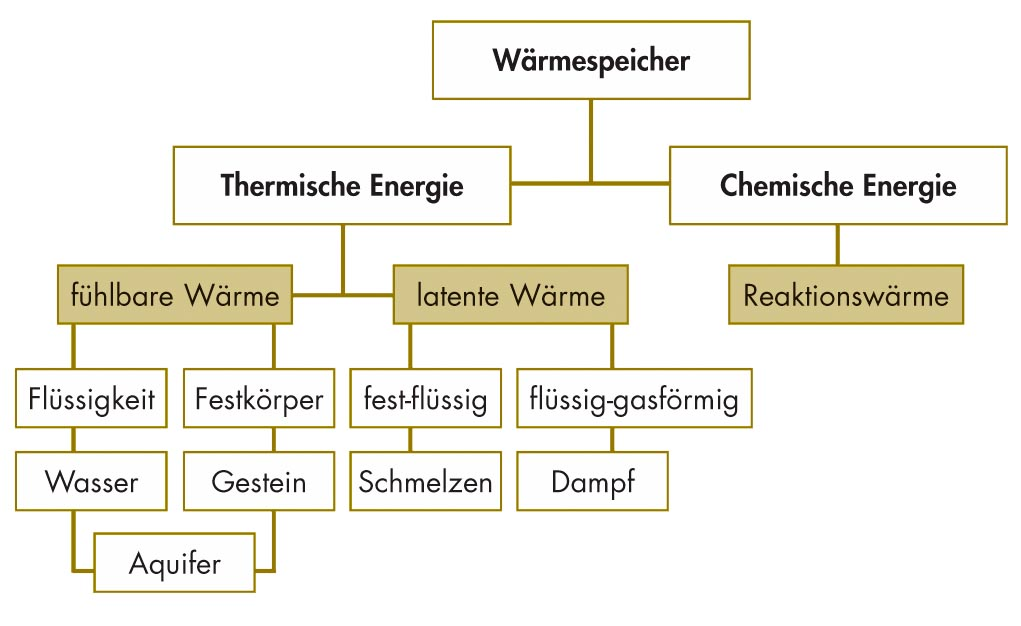
\includegraphics[scale=0.3]{images/speicher.jpg}
\caption{Übersicht über die verschiedenen Wärmespeichertechnolgien \cite{BINE}}
\label{fig:Wärmespeicher}
\end{center}
\end{figure}

\subsection{Chemische Speicher}
test
Chemische Speicher werden über eine chemsiche Reaktion be- und entladen. Per
Definition eines Speichers sind diese Reaktionen reversibel. Die nutzbare
Wärmeenergie entspricht der freigesetzten Reaktionsenthalpie $\Delta
H_{\mathrm{R}}$. Die Nutztemperatur des Speichers bestimmt die in Frage
kommenden chemischen Reaktionen und schränkt die zu verwenden Stoffe erheblich
ein.

Chemische Speicher werden heute im allgemeinen mit sorptiven Prozessen gebaut.
Dies ist einerseits die Adsorption, eine Anlagerung eines Gases oder einer
Flüssigkeit an einen Feststoff und andererseits die Absorption, das Lösen von
Gasen in einer Flüssigkeit. In untenstehender Gleichung ist das Grundlegende
Prinzip der Adsorption erklärt.
\begin{align}
\text{Sorbens}+nH_2O\leftrightharpoons \text{Sorbens}+nH_2O+\Delta H_{ads}
\end{align}
Nutzbar ist die freiwerdende Reaktionsenthalpie $\Delta H_{ads}$ wenn die
Reaktion nach links erfolgt. Die Beladung erfolgt nach umgekehrten Prinzip.
In Abbildung \ref{fig:Sorption} ist ein typischer wasserbasierter
Adsorptionsspeicher dargestellt. Zum Beladen des Speichers wird der desorbierte
Wasserdampf im Kondensator kondensiert. Entladen wird der Speicher mit
niedrigtemperatur Verdampfung von Wasser, der Dampf wird anschliessend an ein
Sorptionsmedium adsorbiert. Dabei wird Hochtemperaturwärme freigesetzt.
\cite{Wesselak}

\begin{figure}[h]
\begin{center}
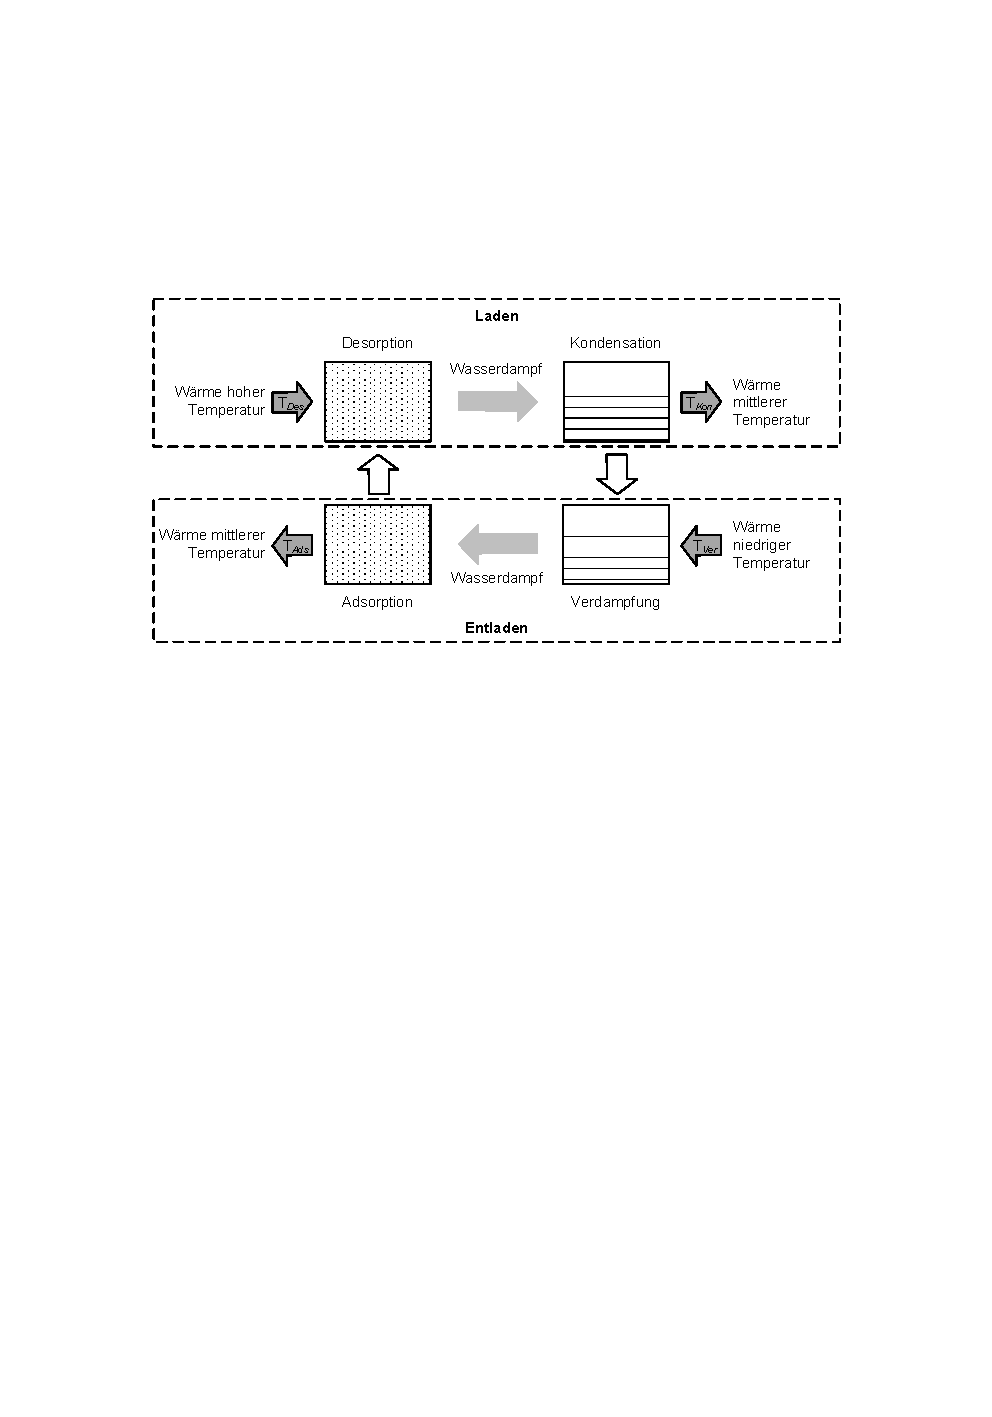
\includegraphics[scale=1]{images/sorption.pdf}
\caption{Prinzip eines geschlossenen wasserbasierten Sorptionsprinzip
\cite{Wesselak}}
\label{fig:Sorption}
\end{center}
\end{figure}
\subsection{Latente Speicher}
Latentwärmespeicher nutzen den Phasenübergang eines Stoffs zur Speicherung von
Wärme. Wie bei den chemischen Speichern beschränken sich die Einsatzgebiete auf
die Phasenübergangseigenschaften des Mediums. Beispielsweise erfolgt der
Phasenübergang von Wasser bei 273.15K. Die freiwerdende bzw. benötigte Energie
für einen fest-flüssig Phasenübergang bei Wasser beträgt 333.5 kJ/kg.
Aufgrund der grossen Dichteänderund der meisten flüssig-gasförmig
Phasenübergänge werden diese selten zu Speicherzwecken genutzt, obwohl die
Kondensations/Verdampfungswärme der Stoffe meistens grösser ist. Die Materialien
werden mit PCM für \flqq Phase Changing Materials\frqq{} abgekürzt.

Die speicherbare Energie ergibt sich nach

\begin{align}
\Delta E = mh_{pc}
\end{align}
Produkt von Masse und Schmelz/Kristallisationsenthalpie. Die verwendeten
Materialien lassen sich zweidimensional anhand der
Schmelz/Kristallationsenthalpie und der Schmelztemperatur kategorisieren. In
Abbildung \ref{fig:Materials} sind einige Materialien die in
Latentwärmespeichern Verwendung finden nach diesen zwei Attributen aufgelistet.

\begin{figure}[h]
\begin{center}
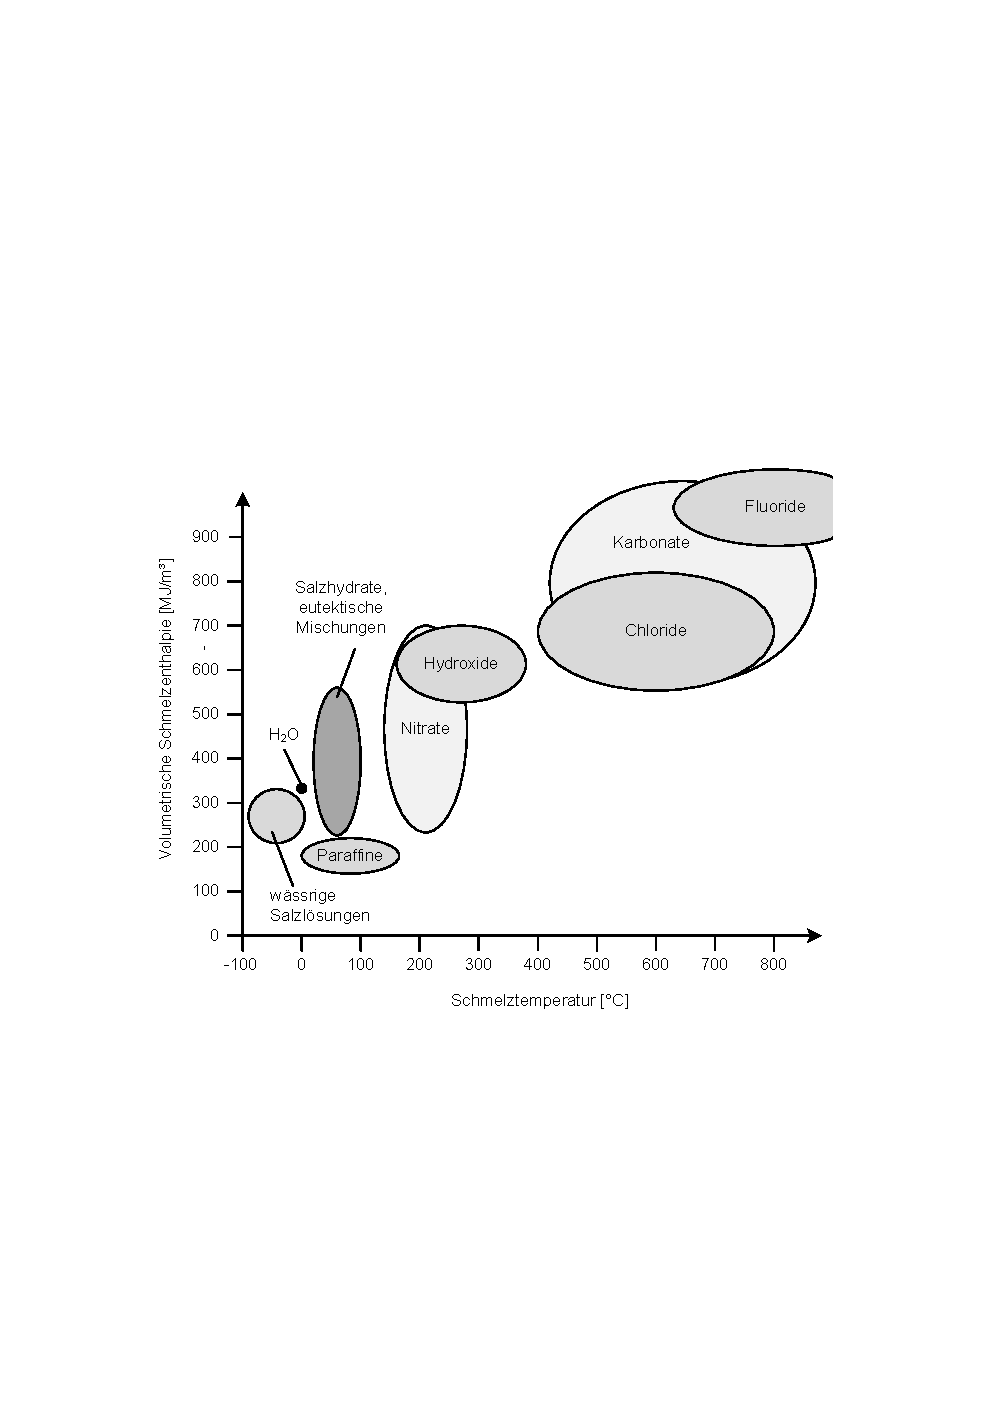
\includegraphics[scale=1]{images/latentmaterial.pdf}
\caption{Kategorisierung von PCM Materialien anhand der Enthlapie und
Temperatur \cite{Hiebler}}
\label{fig:Materials}
\end{center}
\end{figure}

Nachteilig bei Latentwärmespeichern ist besonders, dass bei reinen Feststoffen
naturgemäss kein konvektiver Wärmetransport stattfinden kann. Dem versucht man
im heutigen Forschungskontext mit sogennaten Slurries zu begegnen. Im weiteren
Verlauf dieser Arbeit werden wir darauf noch eingehen. \cite{Wesselak}

\subsection{Sensible Wärmespeicher}

Sensible Wärmespeicher funtkionieren klassisch über eine Temperaturdifferenz
$\Delta T$. Sensibel bedeutet in diesem Kontext \flqq fühlbar\frqq{}. Die
Be- und Entladung funktioniert also über einen \flqq fühlbare\frqq{}
Temperaturdifferenz die über konvektive und konduktive Prozesse zum Austausch
führt. Als Speichermedium eignen sich aufgrund von Dichteeigenschaft und
gewünschter Konvektion verschiedene Flüssigkeiten. Die spezifische
Wärmekapazität $c$ und die Speichermasse $m$ bestimmen die Kapazität des
Speichers, der Massenstrom $\dot{m}$ und Temperaturdifferenz $\Delta T$ die
Leistung des Speichers. Aufgrund der auch an den Speicherwänden anliegenden
Temperaturdifferenz $\Delta T$ ist eine Dämmung zwingend notwendig. 

Technisch gesehen unterscheidet man zwischen Kurz- und Langzeitspeichern.
Typischer Kurzzeitspeicheranwendungen im Gebäudetechnikbereich sind
Warmwasserboiler. Die Verweildauer des Wassers beträgt hier Stunden bis maximal
Tasge. Langzeitspeicher werden zur saisonalen Wärmespeicherung genutzt. Dies
findet beim System Jenni Einsatz. Die Speicher sind so dimensioniert, dass die
SPeicherkapazität nur ein- bis wenige Male im Jahr genutzt wird. Dafür sind aber
grosse Speichermassen, bis zu 100'000l Wasser nötig.

Die gespeicherte Energiemenge lässt sich nach
\begin{align}
\Delta E = mc\Delta T = \rho Vc \Delta T
\end{align}
definieren. Wasser besitzt mit 4.19 kJ/kg/K eine hohe spezifische
Wärmekapazität und wird deshalb als kostengünstiges, effizientes und
umweltfreundliches Medium omnipräsent eingesetzt.
In Abbildung \ref{fig:Langzeitspeicher} sind die verfügbaren
Langzeitsenisbelwärmespicher abgebildet.

\begin{figure}[h]
\begin{center}
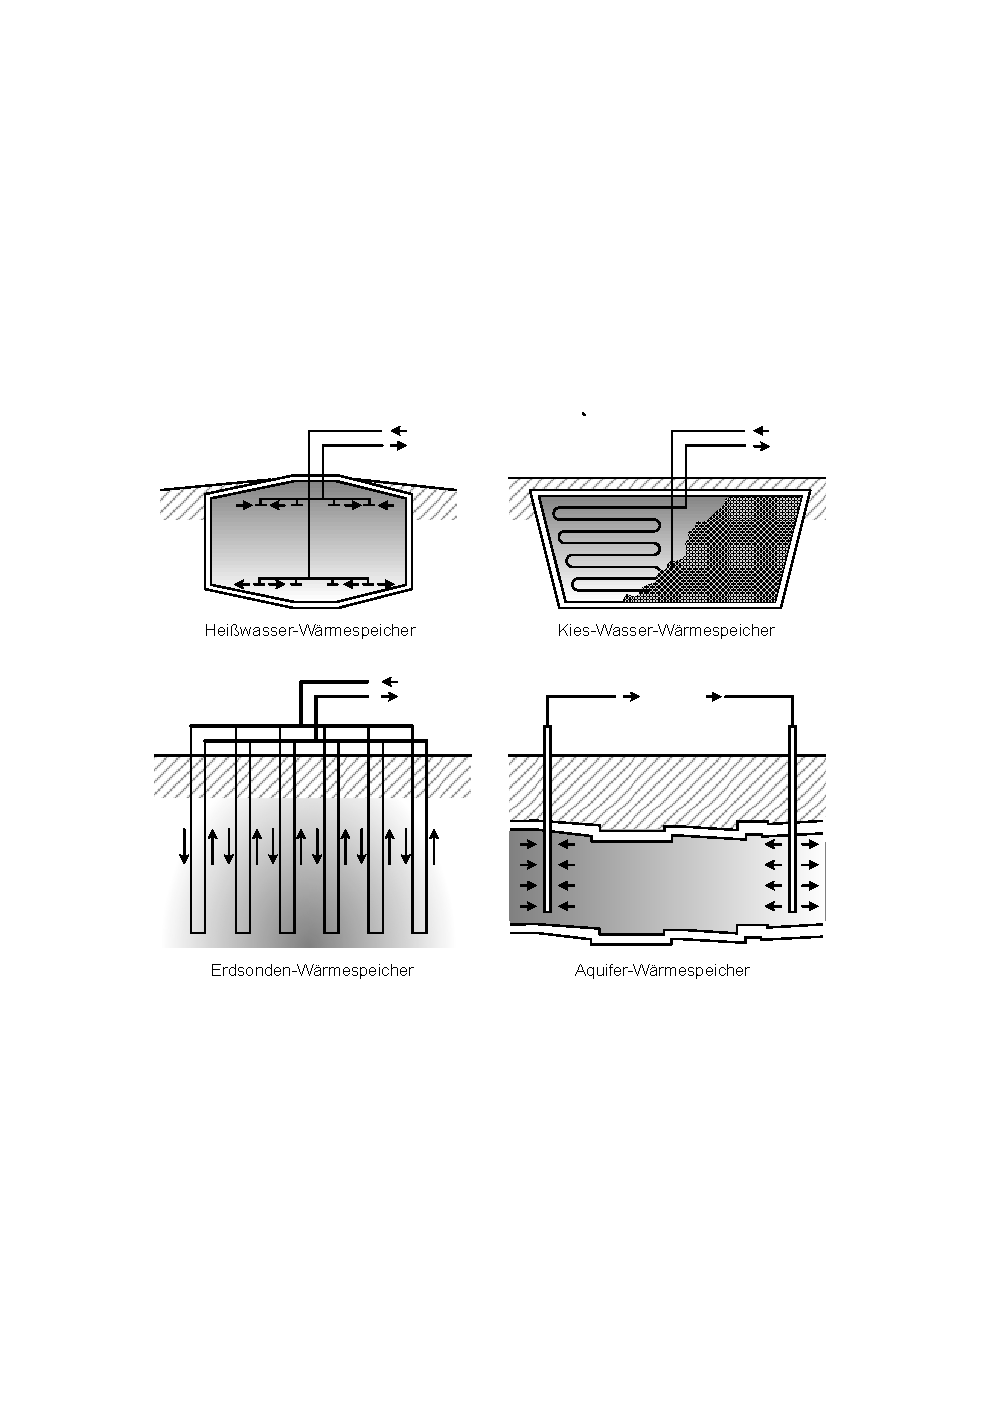
\includegraphics[scale=1]{images/langzeitspeicher.pdf}
\caption{Langzeitsensibelwärmespeicher \cite{Wesselak}}
\label{fig:Langzeitspeicher}
\end{center}
\end{figure}

\section{Technologischer Überblick}
\subsection{Latentspeicher}
\subsubsection{Stand der Technik}
\subsubsection{Entwicklung}
\subsubsection{Perspektiven}
\subsubsection{Chancen}
\subsubsection{Herausforderungen}
\subsection{chemische Speicher}
\subsubsection{Stand der Technik}
\subsubsection{Entwicklung}
\subsubsection{Perspektiven}
\subsubsection{Chancen}
\subsubsection{Herausforderungen}


\newpage
\section{Einsatzgebiete}
\subsection{Latentwärmespeicher}
\subsection{chemische Speicher}

\newpage
\section{Ausblick}

\listoftables
\newpage
\listoffigures
\newpage
\begin{thebibliography}{99}
	\bibitem{BINE}BINE Energieforschung für die Praxis. Abgerufen am 11.04.2014 von
	http://www.bine.info/typo3temp/pics/b193b0972c.gif verändert durch D. Strebel
	\bibitem{Wesselak}Wesselak et. al. Regenerative Energiesysteme. 2. Auflage.
	Springer Vieweg Verlag Berlin. 2013
	\bibitem{Hiebler} Hiebler S. Kalorimetrische Methoden zur Bestimmung der
	Enthalpie von Latentwärmespeichermaterialien während des Phasenübergangs. Dissertation.
	München. 2007
\end{thebibliography}
\end{document}
